\documentclass[tikz,border=6pt]{standalone}
\usepackage{times}
\usetikzlibrary{arrows.meta}
\begin{document}
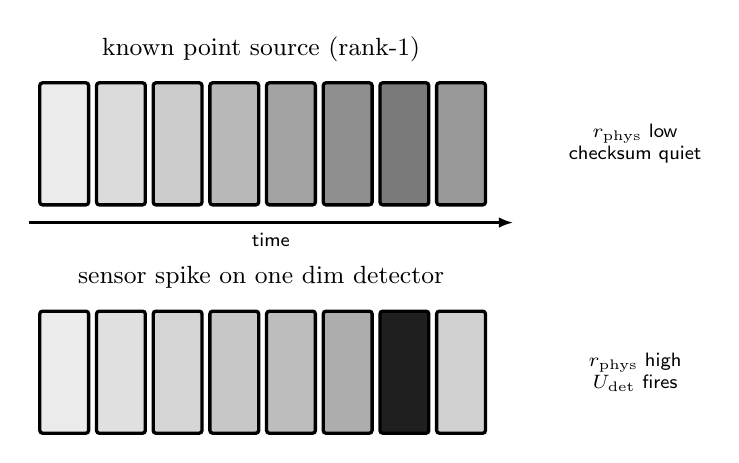
\begin{tikzpicture}[
  font=\sffamily\scriptsize,
  det/.style={draw, very thick, rounded corners=1pt, minimum width=0.62cm, minimum height=1.55cm, inner sep=1pt},
  arr/.style={-{Latex[length=1.8mm]}, thick},
]
\node[font=\small] at (2.5, 2.55) {known point source (rank-1)};
\foreach \x/\f in {0/8, 0.72/14, 1.44/20, 2.16/28, 2.88/36, 3.60/44, 4.32/52, 5.04/40} {
  \node[det, fill=black!\f] at (\x, 1.35) {};
}
\draw[arr] (-0.45, 0.35) -- (5.7, 0.35) node[midway, below] {time};
\node[font=\small] at (2.5, -0.35) {sensor spike on one dim detector};
\foreach \x/\f in {0/8, 0.72/12, 1.44/16, 2.16/22, 2.88/26, 3.60/32, 4.32/88, 5.04/18} {
  \node[det, fill=black!\f] at (\x, -1.55) {};
}
\node[align=center] at (7.25, 1.35) {$r_{\mathrm{phys}}$ low\\checksum quiet};
\node[align=center] at (7.25, -1.55) {$r_{\mathrm{phys}}$ high\\$U_{\mathrm{det}}$ fires};
\end{tikzpicture}
\end{document}
